\begin{figure}
\centering
\caption{How often survey respondents wrote tests for \unsafe code (``Write tests''), how often they audited their dependencies' use of \unsafe code(``Audit dependencies''), and how often participants executed their test cases in Miri if they had used the Miri at least once (``Run in Miri'').}
\label{rq5:tests-and-auditing}
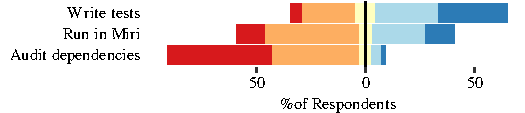
\includegraphics[width=\columnwidth]{figures/compiled/rq5_frequency.pdf}
\vskip 0.5em
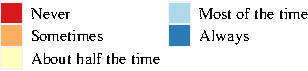
\includegraphics{figures/compiled/legends/legend_frequency_wrapped.pdf}
\end{figure}

Participants used a wide variety of development tools to assist with validating their design choices.

\FPeval{\tested}{round(\ArrayItem{rq5.tests.most.of.the.time} + \ArrayItem{rq5.tests.always}, 0)}
\FPeval{\miritested}{round(\ArrayItem{rq5.miri.test.sometimes} + \ArrayItem{rq5.miri.test.never}, 0)}

\paragraph{Dynamic Analysis} Most participants used dynamic bug-finding tools. Interview participants often mentioned Miri, AddressSanitizer, and Valgrind. Survey respondents most frequently used Miri (\ArrayItemRounded{rq5.tool.miri}\%), Valgrind (\ArrayItemRounded{rq5.tool.valgrind}\%), cargo-fuzz (\ArrayItemRounded{rq5.tool.cargo.fuzz}\%), and AddressSanitizer (\ArrayItemRounded{rq5.tool.addresssanitizer.(asan)}\%). Each remaining tool was used by less than 15\% of survey respondents. Three interview participants and \ArrayItemRounded{rq5.fuzzed}\% of survey respondents used fuzzing tools. One interview participant leveraged industry sponsorship to fuzz a JIT compiler for hours-on-end. Another participant implemented a B-Tree with optimizations for high-performance computing, and they used libFuzzer to perform differential testing~\cite{mckeeman98} against the BTree from Rust's standard library.

A majority (\tested\%) of survey respondents wrote tests for their \unsafe applications at least most of the time. However, Figure~\ref{rq5:tests-and-auditing} shows \miritested\% of participants who had used Miri only sometimes used it to validate their test cases, if at all. This may be due to Miri's lack of support for foreign functions, which was noted by the majority of interview participants. This was also a significant obstacle for survey respondents; \ArrayItemRounded{rq5.miri.deter.lack.of.support.for.foreign.function.calls}\% were deterred from using Miri because it could not call foreign functions. Respondents also avoided using Miri due to its performance (\ArrayItemRounded{rq5.miri.deter.slow.performance}\%) and lack of support for inline assembly (\ArrayItemRounded{rq5.miri.deter.lack.of.support.for.inline.assembly}\%). 
One participant had frequently encountered aliasing violations due to foreign function calls. They circumvented Miri's lack of FFI support by creating mocks of foreign functions, but this solution did not scale to programs with \ilquote{50,000 lines of code}{4} This participant and a few others were aware of the Krabcake project~\cite{krabcake}. Each was already using Valgrind with Rust codebases, and they perceived that Krabcake would be an ideal solution for overcoming each of Miri's limitations.


\FPeval{\debuggedyearly}{round(\ArrayItem{rq5.debugging.yearly} + \ArrayItem{rq5.debugging.less.than.once.a.year} + \ArrayItem{rq5.debugging.never}, 0)}
\FPeval{\debuggedmonthly}{round(\ArrayItem{rq5.debugging.monthly}, 0)}
\FPeval{\debuggeddaily}{round(\ArrayItem{rq5.debugging.daily}, 0)}

\paragraph{Debugging} Few interview participants reported using a debugger with Rust code. Only \debuggeddaily\% of survey respondents used a debugger daily, \debuggedmonthly\% used one monthly, and \debuggedyearly\% used one yearly at most, if at all. One interview participant had used both MSVC's debugger and LLDB, and while both worked, neither matched the quality of the other parts of the Rust toolchain, \ilquote{where you get all the bells and whistles that you want, and things just work nicely together}{3}. Mozilla's RR debugger~\cite{rr_debugger} was useful for one participant to resolve bugs found from fuzzing, but it was generally more common for participants to report using \ilquote{\code{printf}-style}{7} debugging.

\paragraph{Formal Methods} Few interview participants and only \ArrayItemRounded{rq5.formal}\% of survey respondents used tools that apply formal methods for static and dynamic verification. Interview participants mentioned using Kani, Prusti, and Crucible. Kani was useful for one participant, who needed to prove that a particular routine would never execute more than twice for any input. Another participant who had \ilquote{tried a bunch of the tools}{11} in this category found that Prusti was the most complete, but they felt that it would be more effective if these tools were \ilquote{inherently part of Rust}{11} so that they could \ilquote{hoist a lot of currently unsafe code into safe code}{11}. Of the survey respondents who had used formal methods tools, \ArrayItemRounded{rq5.formal.kani}\% had used Kani. Both Prusti and Creusot were used by \ArrayItemRounded{rq5.formal.prusti}\%, and Flux was used by \ArrayItemRounded{rq5.formal.flux}\%.

\FPeval{\noauditing}{round(\ArrayItem{rq5.auditing.frequency.never} + \ArrayItem{rq5.auditing.frequency.sometimes}, 0)}
\FPeval{\auditingtoolpercent}{round(\ArrayItem{rq5.auditing.tools.count} / \ArrayItem{responses.survey.valid} * 100, 0)}
\subsubsection{Auditing} Only a few interview participants described auditing \unsafe code. One participant would typically only examine their dependencies if they were curious about how they functioned. However, they did actively avoid dependencies that used outdated versions of Rust or deprecated features. Another participant was in the process of having a third-party institution examine their codebase to determine if they could reduce the amount of \unsafe code. Survey respondents also rarely audited their dependencies' use of \unsafe code; \noauditing\% audited their dependencies' use of \unsafe less than half the time, as shown in Figure~\ref{rq5:tests-and-auditing}. Additionally, only \auditingtoolpercent\% of respondents had used automated auditing tools. Of this subset, \ArrayItemRounded{rq5.auditing.tools.cargo-audit}\% had used cargo-audit, \ArrayItemRounded{rq5.auditing.tools.cargo-update}\% had used cargo-update, \ArrayItemRounded{rq5.auditing.tools.cargo-deny}\% had used cargo-deny, \ArrayItemRounded{rq5.auditing.tools.cargo-geiger}\% had used cargo-geiger, and only \ArrayItemRounded{rq5.auditing.tools.cargo-vet}\% had used cargo-vet.

\rsqfive Miri, Valgrind, cargo-fuzz, and AddressSanitizer were the most popular dynamic bug-finding tools that developers used with Rust applications. Though Miri was the most commonly used dynamic bug-finding tool, its performance and lack of support for key features deterred developers from using it. Holtervennhoff et al.~\cite{holtervennhoff23} found that developers rarely audit their code; our results illustrate that this is generally true. Developers rarely audited their dependencies' use of \unsafe code, and less than half had used auditing tools. 

